\documentclass[../thesis.tex]{subfiles}
\begin{document}
\chapter{Introduction}\label{cap:introduction}
Improving the way an operator can interact with a robot is a hard challenge in the field of \gls{hri}. The main idea of the project is to solve this problem by using Computer Vision and Machine Learning techniques to recognize some hand gestures made by the operator. In this way, the operator can use the expressive power of his/her hands and their immediacy to communicate with the robot. Moreover, making this idea an interface through the \gls{ros} framework will allow us not to care which robot anyone want to control in the future because it will be enough that it accepts specific messages to work. An example of the idea we want to implement is the one in~\ref{fig:systemArchitecture}.

\begin{figure}[H]
  \centering
  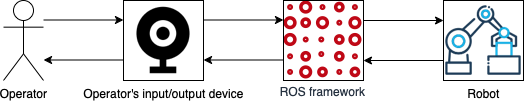
\includegraphics[width=0.7\columnwidth]{systemArchitecture.png}
  \caption{Example of system archicture.}
  \label{fig:systemArchitecture}
\end{figure}

\section{Motivation and objectives}\label{s:motivation-and-objectives}


\section{Organization}\label{s:organization}

\end{document}
